% Cardiac arrest early warning pipeline: manuscript draft
% Target: Springer Nature venue (adapt this preamble to the svjour3 template
% when submitting; content sections transfer unchanged).
% Style note: no hyphens or dashes anywhere in the prose of this document.

\documentclass[11pt]{article}

\usepackage[utf8]{inputenc}
\usepackage[T1]{fontenc}
\usepackage{amsmath}
\usepackage{graphicx}
\usepackage{booktabs}
\usepackage{caption}
\usepackage[hidelinks]{hyperref}
\usepackage{algorithm}
\usepackage{algpseudocode}
\usepackage{tikz}
\usetikzlibrary{positioning}
\usepackage[a4paper,margin=1in]{geometry}

\title{A Multimodal Early Warning Pipeline for Cardiac Arrest Using Foundation Model Embeddings}
\author{[Author names to be added]}
\date{\today}

\begin{document}

\maketitle

\begin{abstract}
We present a complete, reproducible pipeline that scores the risk of cardiac arrest
within the next 1, 6 or 24 hours from bedside monitor signals: electrocardiogram,
photoplethysmogram, arterial blood pressure and heart rate. Two open foundation
models, ECG FM (a wav2vec 2.0 style model with 90.9 million parameters) and PaPaGei S,
summarize the raw waveforms into embeddings, and a temporal network in the Wav2Arrest
style (bidirectional LSTM with learned attention) consumes a 6 hour history of fused
features to produce per horizon risk estimates and a time to event estimate.
The pipeline was validated end to end on a synthetic cohort of 60 patients with 28
arrest events, where it reached a 6 hour AUROC of 0.891 on held out patients with a
first true alert 21.7 hours before arrest. A stress test on the open access Sudden
Cardiac Death Holter Database produced a genuine negative result: the synthetic
trained model does not transfer to real data, and no model variant trained on 20
real patients beats chance at 6 hours, including identity adversarial training and
three alternative fusion schemes with explicit missing modality masks. At 1 hour a
weak signal exists and comes from engineered rate features rather than the
foundation model embeddings. We discuss why this outcome is expected for Holter
data without hemodynamic signals, and identify the credentialed MIMIC III
evaluation as the decisive next step. This report is a research prototype and makes
no clinical claim.
\end{abstract}

\section{Introduction}
Cardiac arrest in hospital often follows hours of measurable hemodynamic
deterioration, which makes early warning a promising target for machine learning on
continuous monitor data. Wav2Arrest and its successor introduced a strong recipe for
this task: a foundation model feature extractor, a temporal aggregator, time to
event targets and patient level evaluation. We follow that recipe and extend it to
four signal modalities.

The contribution of this work is an open, reproducible implementation of the full
chain: data, labels, preprocessing, engineered features, embeddings from two real
foundation models, a temporal risk model, an alert simulator and a strict
evaluation protocol. We report results on a physiologically coupled synthetic
cohort and on the only open access real pre arrest dataset, the Sudden Cardiac
Death Holter Database. Both results are reported honestly: the synthetic numbers
validate the machinery, and the real data test currently fails, which we analyze
rather than hide.

\section{Methodology}

\subsection{Pipeline overview}
Figure~\ref{fig:flow} shows the pipeline. Signals are resampled to a common 125 Hz
clock and cut into 5 minute windows. Each window receives three feature blocks:
engineered features computed from the waveforms, an ECG FM embedding and a
PaPaGei S embedding. The fused vector feeds a temporal network that watches the
last 6 hours and outputs three risk scores plus a time to event estimate. Alerts
fire when the 6 hour risk crosses a threshold, subject to a refractory period.

\begin{figure}[t]
\centering
\resizebox{\textwidth}{!}{
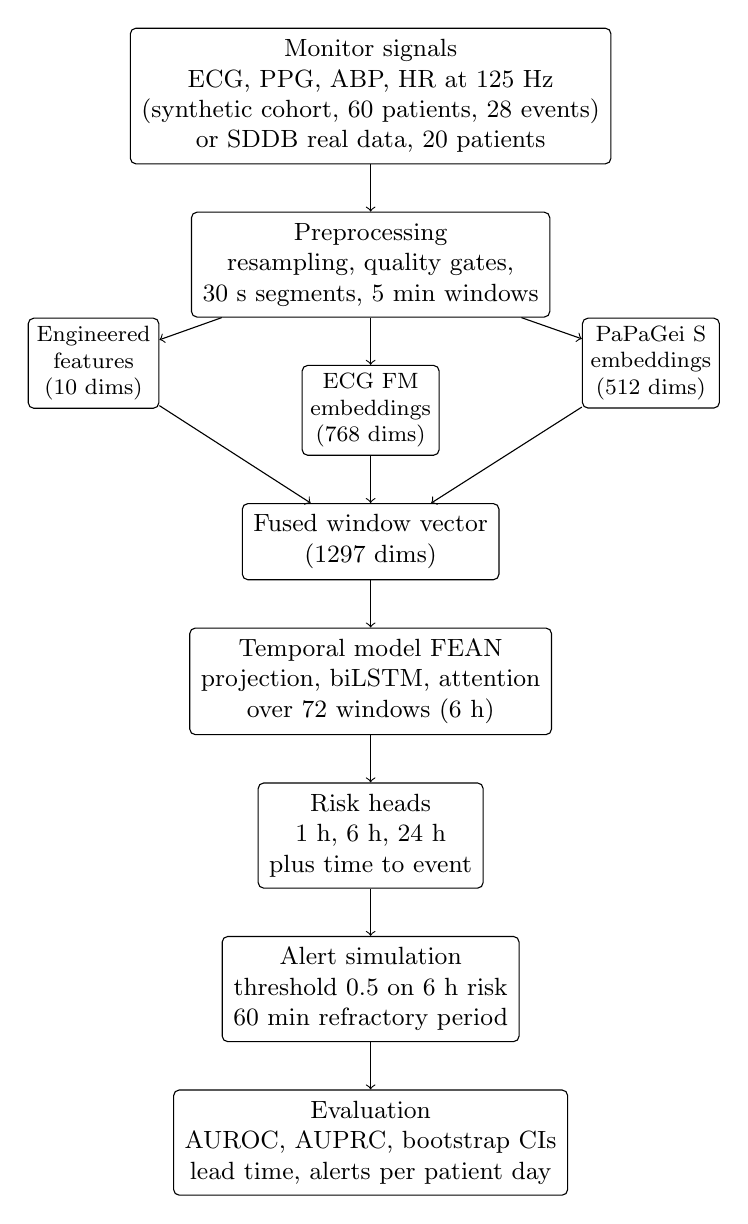
\begin{tikzpicture}[
    node distance=6mm,
    block/.style={draw, rounded corners=2pt, align=center, font=\small, inner sep=4pt},
    small/.style={draw, rounded corners=2pt, align=center, font=\footnotesize, inner sep=3pt}
]
\node[block] (a) {Monitor signals \\ ECG, PPG, ABP, HR at 125 Hz \\ (synthetic cohort, 60 patients, 28 events) \\ or SDDB real data, 20 patients};
\node[block, below=of a] (b) {Preprocessing \\ resampling, quality gates, \\ 30 s segments, 5 min windows};
\node[small, below left=0mm and 4mm of b] (c1) {Engineered \\ features \\ (10 dims)};
\node[small, below=of b] (c2) {ECG FM \\ embeddings \\ (768 dims)};
\node[small, below right=0mm and 4mm of b] (c3) {PaPaGei S \\ embeddings \\ (512 dims)};
\node[block, below=of c2] (d) {Fused window vector \\ (1297 dims)};
\node[block, below=of d] (e) {Temporal model FEAN \\ projection, biLSTM, attention \\ over 72 windows (6 h)};
\node[block, below=of e] (f) {Risk heads \\ 1 h, 6 h, 24 h \\ plus time to event};
\node[block, below=of f] (g) {Alert simulation \\ threshold 0.5 on 6 h risk \\ 60 min refractory period};
\node[block, below=of g] (h) {Evaluation \\ AUROC, AUPRC, bootstrap CIs \\ lead time, alerts per patient day};
\draw[->] (a) -- (b);
\draw[->] (b) -- (c1);
\draw[->] (b) -- (c2);
\draw[->] (b) -- (c3);
\draw[->] (c1) -- (d);
\draw[->] (c2) -- (d);
\draw[->] (c3) -- (d);
\draw[->] (d) -- (e);
\draw[->] (e) -- (f);
\draw[->] (f) -- (g);
\draw[->] (g) -- (h);
\end{tikzpicture}
}
\caption{Pipeline overview: signals, preprocessing, three feature blocks, the
temporal model FEAN, alert simulation and evaluation.}
\label{fig:flow}
\end{figure}

\subsection{Synthetic cohort generation}
The synthetic cohort produces monitor style signals with physiological coupling so
that every later stage has a learnable, quality checked input. Beat trains are
generated for the electrocardiogram (P, QRS and T waves as Gaussian bumps), and
each R peak is followed by a photoplethysmogram pulse and an arterial pressure
pulse delayed by the pulse transit time, which lengthens as blood pressure falls.
Arrest patients receive a 6 hour drift: rising heart rate, falling blood pressure
and oxygen saturation, falling heart rate variability and rising pulse transit
time. Quality defects (flatline, saturation, noise bursts) are injected in five
percent of stream windows, and ten percent of patients lack the
photoplethysmogram stream. Algorithm~\ref{alg:cohort} summarizes the generator.

\begin{algorithm}[t]
\caption{Synthetic cohort generation}
\label{alg:cohort}
\begin{algorithmic}[1]
\State \textbf{Inputs:} patient count $N$, arrest fraction $p$, stay length range, drift window $D$
\For{each patient $i$ in $1 \dots N$}
    \State draw stay length and admission time
    \State mark case with probability $p$; if case, draw arrest time inside stay
    \For{each 5 min window $w$ in stay}
        \State draw baseline vitals (heart rate, pressures, saturation) with wander and noise
        \If{case and window inside last $D$ hours before arrest}
            \State apply drift: heart rate up, pressures and saturation down, transit time up
        \EndIf
        \If{case and window after arrest}
            \State mark window excluded (post arrest)
        \EndIf
        \State draw quality flag per stream (ok, flat, sat, noise)
    \EndFor
\EndFor
\State \textbf{return} vitals table, event table
\end{algorithmic}
\end{algorithm}

\subsection{Cohort and labels}
For each horizon $H \in \{1, 6, 24\}$ hours, a window receives a binary label that
is 1 when the arrest occurs within the next $H$ hours, together with a time to
event target in hours for case patients. Windows during or after resuscitation are
excluded, as are windows in the final 15 minutes before arrest, when clinicians are
already responding. Excluded windows keep their row with a reason field so that
downstream code can assert the exclusion. Algorithm~\ref{alg:labels} gives the
procedure.

\begin{algorithm}[t]
\caption{Window labeling and exclusions}
\label{alg:labels}
\begin{algorithmic}[1]
\For{each patient and each 5 min window}
    \If{window ends after arrest time}
        \State mark excluded, label missing \Comment{post arrest}
    \ElsIf{window ends within 15 min of arrest}
        \State mark excluded, label missing \Comment{response phase}
    \Else
        \For{each horizon $H$ in 1, 6, 24 hours}
            \State label is 1 if time to arrest is at most $H$ hours, else 0
        \EndFor
        \State time to event equals arrest time minus window end time (cases only)
    \EndIf
\EndFor
\end{algorithmic}
\end{algorithm}

\subsection{Preprocessing and quality control}
All streams share one clock at 125 Hz. Resampling to encoder targets uses linear
interpolation for upsampling (the ECG FM preprocessing does the same) and
polyphase filtering for decimation. Each stream passes a rule based gate: flatline
(standard deviation below threshold), saturation (fraction of samples pinned at the
rails), and a signal to noise heuristic (physiological band power versus high
frequency band power). Segments of 30 seconds are cut deterministically per patient
and window, so embeddings can be cached and recomputed without drift.
Algorithm~\ref{alg:gate} states the gate. Splits are patient level at all times:
no patient appears in more than one of train, validation and test.

\begin{algorithm}[t]
\caption{Per stream quality gate}
\label{alg:gate}
\begin{algorithmic}[1]
\State \textbf{Inputs:} segment $x$, rate $fs$
\If{all samples missing}
    \State \textbf{return} fail (missing stream)
\EndIf
\If{standard deviation of $x$ below flat threshold}
    \State \textbf{return} fail (flatline)
\EndIf
\State saturation flag if pinned fraction above threshold
\State signal power in 0.5 to 12 Hz band, noise power in 30 to 60 Hz band
\State low ratio flag if signal to noise ratio below threshold
\State \textbf{return} pass if no flag raised, else fail with flags
\end{algorithmic}
\end{algorithm}

\subsection{Engineered features}
Each window receives ten engineered features computed from its waveforms: heart
rate variability (mean RR interval, SDNN, RMSSD), ectopy burden as the fraction of
premature RR intervals, arterial pressure mean and variability, the pulse transit
time estimated per beat as the delay from each R peak to the steepest upstroke of
the following photoplethysmogram pulse (median over beats), a quality pass
indicator, and 30 minute trends of heart rate and systolic pressure from the
vitals table. On the synthetic cohort the estimated transit time correlates with
the ground truth at 0.979. Algorithm~\ref{alg:features} lists the computation.

\begin{algorithm}[t]
\caption{Engineered features per window}
\label{alg:features}
\begin{algorithmic}[1]
\State detect R peaks in the 30 s electrocardiogram
\State RR intervals; mean RR, SDNN, RMSSD, ectopy fraction
\State arterial pressure mean and variability from the pressure waveform
\For{each R peak}
    \State take the photoplethysmogram window from 30 ms to 550 ms after the peak
    \State foot equals position of steepest upstroke in that window
    \State delay equals foot position in milliseconds
\EndFor
\State transit time equals median delay over beats
\State join 30 minute heart rate and pressure trends from the vitals table
\State \textbf{return} ten feature values
\end{algorithmic}
\end{algorithm}

\subsection{Foundation model embeddings}
Two frozen foundation models summarize the waveforms. ECG FM expects 12 leads at
500 Hz in 5 second segments and returns 768 dimensional embeddings; the single
monitor lead is placed in the lead II slot and the remaining leads are zero
filled, which mirrors reduced lead use at the bedside. PaPaGei S expects
10 second photoplethysmogram segments at 125 Hz and returns 512 dimensional
embeddings. The two encoders require conflicting Python environments, so each runs
in a dedicated conda environment invoked by subprocess, and every embedding is
cached on disk. Segment embeddings are mean pooled to the 5 minute window level.
Algorithm~\ref{alg:embed} describes the orchestration.

\begin{algorithm}[t]
\caption{Embedding extraction}
\label{alg:embed}
\begin{algorithmic}[1]
\For{each 5 min window}
    \State cut the 30 s segment, resample to encoder rate, z score
    \State electrocardiogram: map lead to slot II, zero fill, 5 s chunks
    \State photoplethysmogram: 10 s chunks
\EndFor
\For{each encoder in (ECG FM, PaPaGei S)}
    \State run extractor via subprocess in its dedicated environment
    \State cache segment embeddings on disk
\EndFor
\State mean pool segment embeddings per window
\end{algorithmic}
\end{algorithm}

\subsection{Temporal risk model}
The model follows the FEAN design of Wav2Arrest. Each window vector (7 vitals,
10 engineered, 768 electrocardiogram, 512 photoplethysmogram, 1297 in total) is
projected to a hidden size, processed by a two layer bidirectional LSTM over the
last 72 windows (6 hours) with packing for variable lengths, pooled by learned
attention with a padding mask, and mapped by linear heads to three risk logits and
a normalized time to event logit. Training minimizes weighted binary cross entropy
per horizon (weights inverse to class frequency) plus mean squared error on the
time to event head for positive windows. Algorithm~\ref{alg:fean} gives the
forward pass and loss.

Two extensions address generalization and fusion. First, an identity adversarial
head (gradient reversal against a patient ID classifier on the context vector,
ramped in over five epochs) discourages the representation from encoding patient
identity, optionally combined with PCGrad, which projects conflicting task
gradients onto each other's normal planes. Second, a fusion comparison replaces
the single concatenation projection with per modality projectors followed by one
of: hierarchical gated fusion, per window modality attention, or static learned
per modality weights. Each modality carries an explicit presence mask; absent
blocks are routed to learned per modality missing embeddings instead of being
treated as zero valued data. On the synthetic cohort the fusion variants match the
concatenation baseline within noise (6 hour AUROC 0.77 to 0.86), and with the
photoplethysmogram removed at evaluation time gated and weighted fusion remain
stable while attention fusion degrades; the identity adversarial variants are
sanity checked there as well (no NaNs, losses decrease, and the identity probe
stays high by construction because case and control are patient level properties
on synthetic data).

\begin{algorithm}[t]
\caption{FEAN forward pass and training loss}
\label{alg:fean}
\begin{algorithmic}[1]
\State \textbf{Forward:}
\State project each window vector to hidden size, apply dropout
\State pack sequences, run two layer bidirectional LSTM
\State attention scores with padding masked to minus infinity
\State context vector equals attention weighted mean
\For{each horizon $H$ in 1, 6, 24}
    \State risk logit equals linear head applied to context
\EndFor
\State time to event logit equals linear head applied to context
\State \textbf{Loss:}
\State weighted binary cross entropy with logits per horizon, summed
\State plus mean squared error on time to event for positive windows
\end{algorithmic}
\end{algorithm}

\subsection{Alert simulation and evaluation}
Evaluation streams each held out patient in time order, as a bedside monitor
would. An alert fires when the 6 hour risk reaches 0.5, and no further alert may
fire within 60 minutes (refractory period). Metrics are AUROC, AUPRC and Brier per
horizon with patient level bootstrap confidence intervals (1000 resamples), PPV at
fixed sensitivity, sensitivity at a fixed alert budget, alerts per patient day,
lead time of true alerts, calibration and the time averaged AUC across lead time
bins (0 to 1, 1 to 6, 6 to 24 hours). Algorithms~\ref{alg:sim} and
\ref{alg:boot} state the simulation and the bootstrap.

\begin{algorithm}[t]
\caption{Alert replay simulation}
\label{alg:sim}
\begin{algorithmic}[1]
\For{each window of a patient in time order}
    \State append standardized features to history, keep last 72 windows
    \State compute risk for the alert horizon
    \If{risk above threshold and time since last alert above refractory}
        \State raise alert, record time and risk
    \EndIf
\EndFor
\end{algorithmic}
\end{algorithm}

\begin{algorithm}[t]
\caption{Patient level bootstrap}
\label{alg:boot}
\begin{algorithmic}[1]
\Repeat
    \State resample patients with replacement
    \State restrict windows to sampled patients
    \If{both classes present}
        \State compute the metric on the restricted set
    \EndIf
\Until{1000 iterations done}
\State confidence interval equals the 2.5 and 97.5 percentiles
\end{algorithmic}
\end{algorithm}

\section{Results}

\subsection{Synthetic validation}
Table~\ref{tab:baselines} compares the baselines and the temporal model on the
patient level validation split. Table~\ref{tab:mews} reports the MEWS style score
built from the streams we have (heart rate, systolic pressure, saturation;
respiratory rate, temperature and consciousness are missing and stated as such).
Table~\ref{tab:replay} reports the held out replay evaluation, Table~\ref{tab:alerts}
the alert level metrics, and Table~\ref{tab:ablation} the feature block ablations.

\begin{table}[t]
\centering
\caption{Model performance on the patient level validation split (AUROC).}
\label{tab:baselines}
\begin{tabular}{lccc}
\toprule
Model & 1 h & 6 h & 24 h \\
\midrule
Logistic regression & 1.000 & 0.954 & 0.689 \\
Gradient boosting & 0.998 & 0.993 & 0.911 \\
FEAN temporal model & 1.000 & 0.844 & 0.667 \\
\bottomrule
\end{tabular}
\end{table}

\begin{table}[t]
\centering
\caption{MEWS style score alert statistics on the validation split.}
\label{tab:mews}
\begin{tabular}{lccccc}
\toprule
Threshold & Rate per day & \multicolumn{2}{c}{1 h} & \multicolumn{2}{c}{6 h} \\
 & & Sens. & PPV & Sens. & PPV \\
\midrule
4 & 11.2 & 0.82 & 0.82 & 1.00 & 1.00 \\
5 & 8.1 & 1.00 & 1.00 & 1.00 & 1.00 \\
\bottomrule
\end{tabular}
\end{table}

\begin{table}[t]
\centering
\caption{Held out replay evaluation (two patients, patient level bootstrap CIs).}
\label{tab:replay}
\begin{tabular}{lcccc}
\toprule
Horizon & Positives & AUROC [95\% CI] & AUPRC & Brier \\
\midrule
1 h & 12 & 1.000 [1.000, 1.000] & 1.000 & 0.025 \\
6 h & 72 & 0.891 [0.825, 0.922] & 0.785 & 0.315 \\
24 h & 288 & 0.946 [0.944, 0.948] & 0.976 & 0.137 \\
\bottomrule
\end{tabular}
\end{table}

\begin{table}[t]
\centering
\caption{Alert level metrics on the held out replay patients.}
\label{tab:alerts}
\begin{tabular}{lc}
\toprule
Metric & Value \\
\midrule
First true alert before arrest & 21.7 h \\
Lead time of true alerts (min, median, max) & 0.6, 11.2, 21.7 h \\
False alarms on the control patient & 5 in 24 h (4.9 per patient day) \\
PPV at sensitivity 0.8 (1 h, 6 h, 24 h) & 1.000, 0.307, 1.000 \\
Sensitivity at 1 alert per day (1 h, 6 h, 24 h) & 1.000, 1.000, 1.000 \\
Time averaged AUC across lead time bins & 0.890 \\
\bottomrule
\end{tabular}
\end{table}

\begin{table}[t]
\centering
\caption{Feature block ablations (validation AUROC, 20 epochs each).}
\label{tab:ablation}
\begin{tabular}{lcccc}
\toprule
Variant & 1 h & 6 h & 24 h & Replay alerts (case, control) \\
\midrule
Full & 1.000 & 0.859 & 0.619 & 247, 1 \\
Vitals only & 1.000 & 0.755 & 0.555 & 38, 0 \\
Vitals plus engineered & 1.000 & 0.845 & 0.718 & 51, 0 \\
Vitals plus embeddings & 1.000 & 0.816 & 0.574 & 245, 0 \\
\bottomrule
\end{tabular}
\end{table}

The synthetic results validate the machinery. They are inflated by design: the
drift is deterministic, and the 1 hour horizon is trivially separable. The numbers
must not be read as clinical evidence.

Figures~\ref{fig:drift} to \ref{fig:calib} illustrate the synthetic regime.
Figure~\ref{fig:drift} shows the pre arrest drift, Figure~\ref{fig:waves} one
clean window and the same window with an injected noise artifact rejected by the
quality gate, Figure~\ref{fig:traj} the held out risk trajectories with alerts,
and Figure~\ref{fig:calib} the calibration curves.

\begin{figure}[t]
\centering
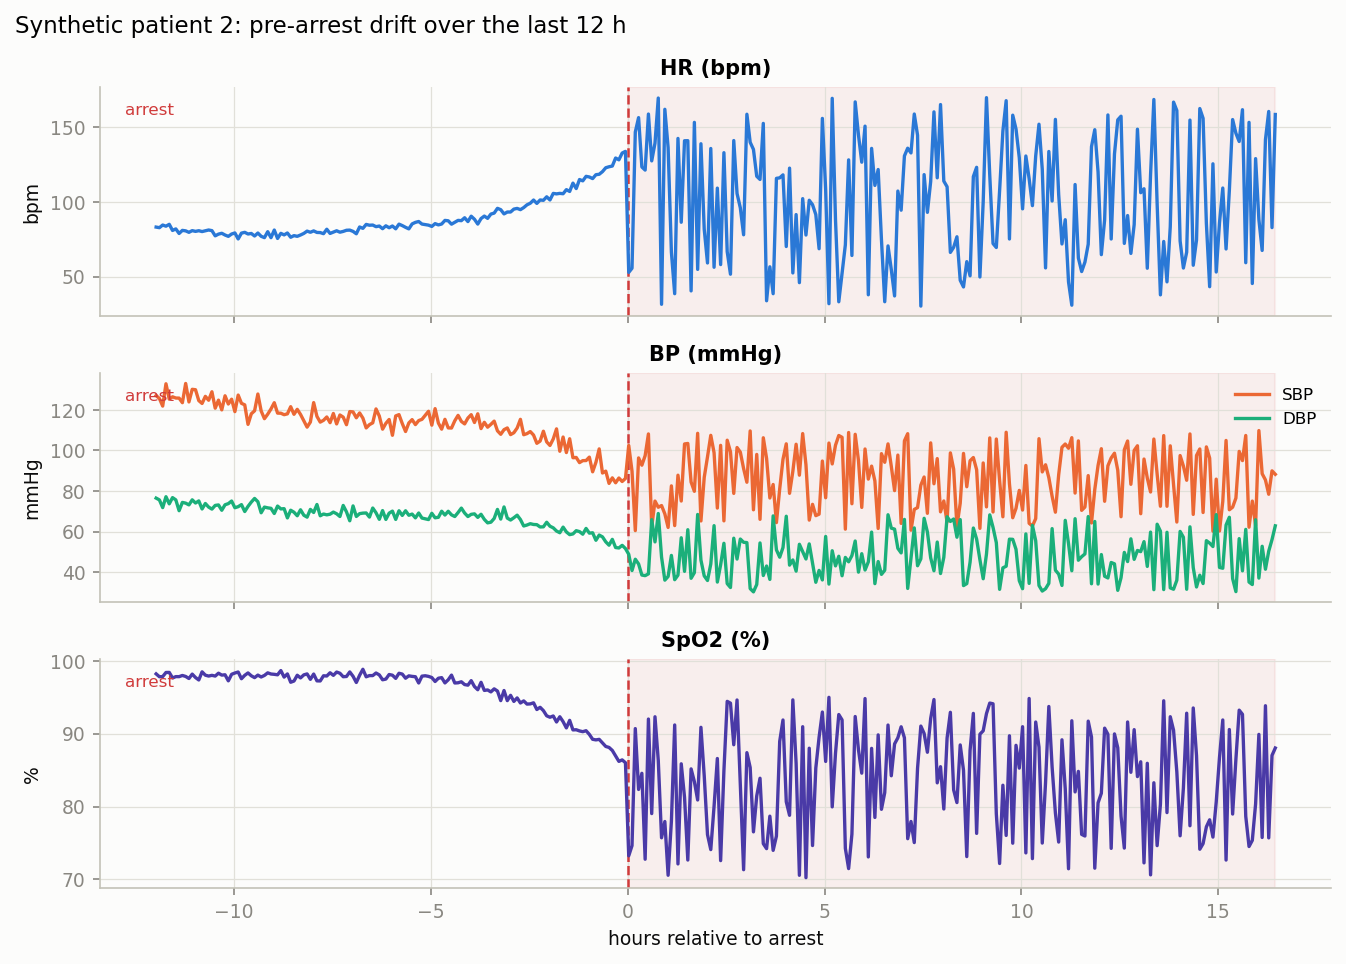
\includegraphics[width=\linewidth]{images/fig01_synthetic_drift.png}
\caption{Pre arrest drift of one synthetic case patient over the last 12 hours
before arrest (heart rate, blood pressure, saturation). The post arrest region is
shaded and excluded downstream.}
\label{fig:drift}
\end{figure}

\begin{figure}[t]
\centering
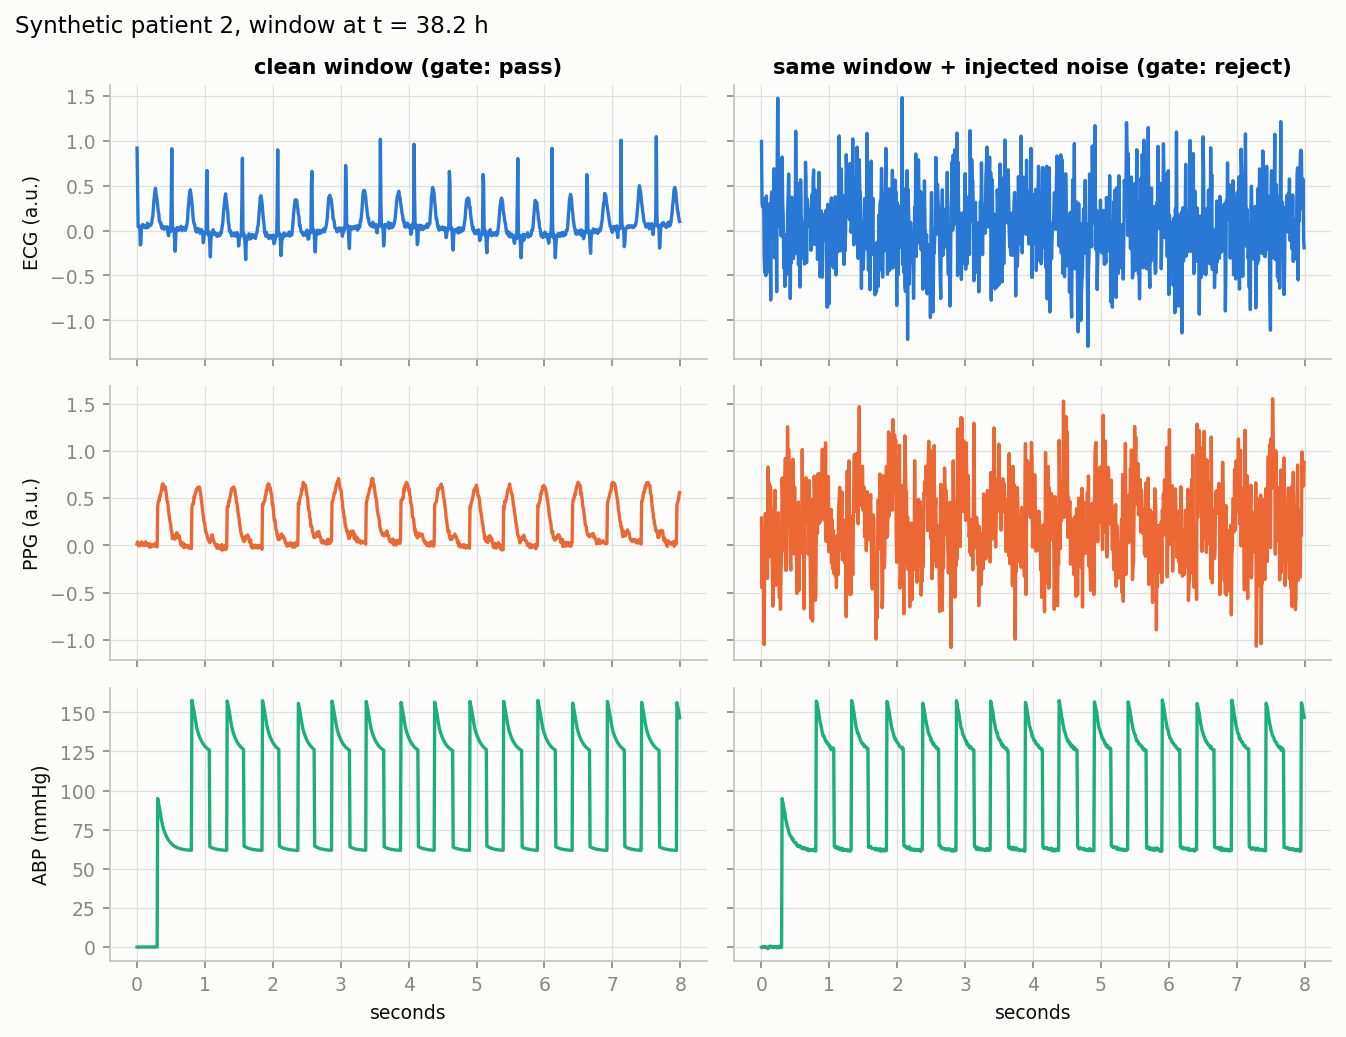
\includegraphics[width=\linewidth]{images/fig02_synthetic_waveforms.png}
\caption{One 30 second window: clean electrocardiogram, photoplethysmogram and
arterial pressure (left) versus the same window with an injected noise artifact
(right), which the quality gate rejects.}
\label{fig:waves}
\end{figure}

\begin{figure}[t]
\centering
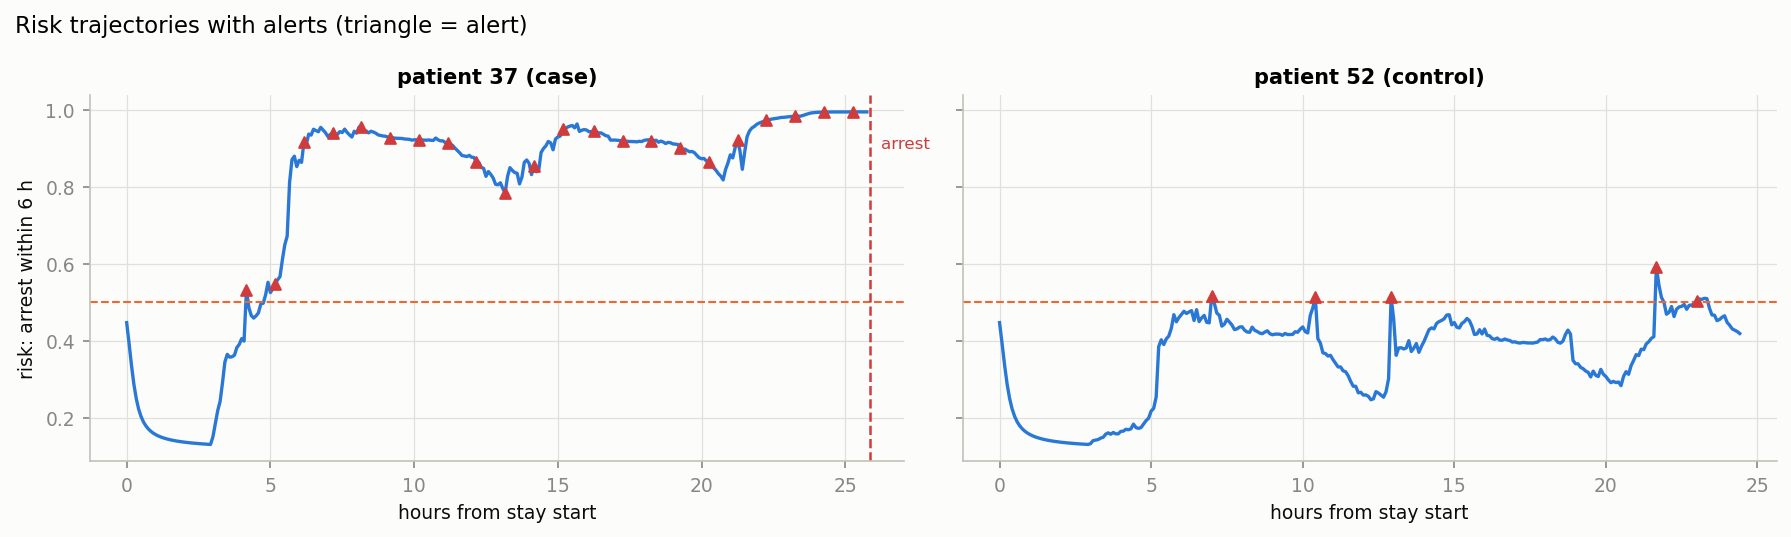
\includegraphics[width=\linewidth]{images/fig03_risk_trajectories.png}
\caption{Risk trajectories of the trained pipeline on the two held out patients.
Triangles mark alerts, the dashed line is the threshold. The case patient (left)
first crosses the threshold about 21 hours before arrest; the control (right)
produces a small number of false alarms.}
\label{fig:traj}
\end{figure}

\begin{figure}[t]
\centering
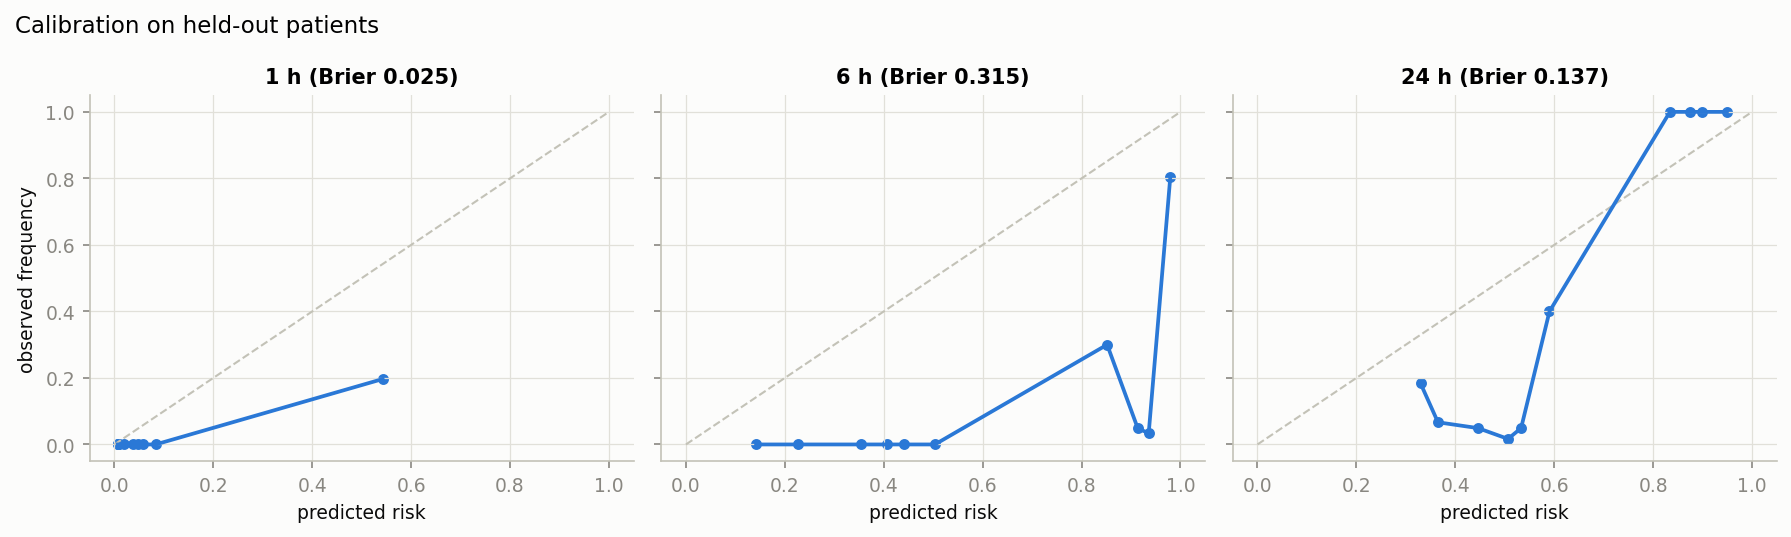
\includegraphics[width=\linewidth]{images/fig04_calibration.png}
\caption{Calibration curves per horizon on the held out patients. Predicted risk
versus observed frequency; the diagonal is perfect calibration.}
\label{fig:calib}
\end{figure}

\subsection{Real data stress test}
The open access Sudden Cardiac Death Holter Database provides 23 two lead 250 Hz
Holter recordings of 4 to 25 hours from patients who arrested during recording;
20 records carry a documented ventricular fibrillation onset time used as the
arrest timestamp. We embedded 1829 five minute windows (the 24 hour horizon is not
evaluable because no recording extends far enough before onset to supply 24 hour
negatives) and ran a zero shot application of the synthetic trained model plus a
5 fold cross validation grouped by patient, for the baseline model, two identity
adversarial variants, and three fusion variants with explicit missing modality
masks. A protocol fix matters: in an earlier version, sequence histories crossed
record and span boundaries, which confounded the results; all numbers below use
the corrected protocol (histories stay inside one record and one span, fixed
seeds) with patient level bootstrap confidence intervals. Table~\ref{tab:sddb}
reports the result.

\begin{table}[t]
\centering
\caption{Real data stress test on the Sudden Cardiac Death Holter Database
(20 patients, 1829 windows; patient level bootstrap CIs).}
\label{tab:sddb}
\begin{tabular}{lcc}
\toprule
Model & 1 h AUROC & 6 h AUROC \\
\midrule
Zero shot (synthetic trained model) & 0.338 & 0.447 \\
FEAN, concatenation (baseline) & 0.632 [0.516, 0.748] & 0.402 [0.344, 0.456] \\
FEAN, identity adversarial & 0.697 [0.599, 0.792] & 0.436 [0.368, 0.501] \\
FEAN, identity adversarial + PCGrad & 0.663 [0.557, 0.781] & 0.459 [0.382, 0.537] \\
FEAN, gated fusion + masks & 0.655 [0.546, 0.778] & 0.386 [0.337, 0.435] \\
FEAN, modality attention + masks & 0.638 [0.519, 0.754] & 0.473 [0.402, 0.538] \\
FEAN, static modality weights + masks & 0.660 [0.546, 0.776] & 0.394 [0.347, 0.443] \\
Ablation: engineered features only & 0.767 [0.705, 0.837] & 0.508 [0.461, 0.555] \\
Ablation: embeddings only & 0.707 [0.602, 0.812] & 0.422 [0.377, 0.462] \\
Slow risk layer (3 h blocks, QT/TWA/HRV, LR) & 0.426 [0.193, 0.667] & 0.313 [0.190, 0.400] \\
\bottomrule
\end{tabular}
\end{table}

We verified that this is a genuine negative result and not a training failure:
train loss decreases across epochs while held out loss stays flat, and
predictions spread widely, yet held out records remain at or below chance at
6 hours for every variant; on one fold several variants become confidently
inverted (AUROC near zero), learning record specific patterns that do not
transfer across 16 training patients. Figures~\ref{fig:sddb} and
\ref{fig:curves} show one real patient trajectory and the learning curves.

Three variant level lessons. First, the models do recognize patients: a linear
identity probe on the context vector classifies held out train windows into
patients at 0.13 to 0.47 accuracy across variants (chance 0.05), so leakage is
present and quantified. The identity signal is carried by the embedding block
(probe 0.439 without engineered features versus 0.130 without embeddings).
Identity adversarial training helps slightly at both horizons but does not
reduce the probe (0.423 to 0.470), so gradient reversal does not remove the
leakage; modality attention is the only architecture that substantially
reduces it (probe 0.143), and it is also the best held out variant at 6 hours.
Second, concatenation, gating and static weights are statistically
indistinguishable; modality attention is the best deep variant at 6 hours but
also the least stable. Missing modality masks keep predictions finite when
streams disappear but do not change the ranking. Third, the 1 hour signal is
carried by engineered heart rate variability and ectopy features (0.767
without embeddings), and the ECG FM embeddings dilute it (0.632 full model).
Attention salience shows the model spreads its attention over history and puts
near zero weight on the current window.

\begin{figure}[t]
\centering
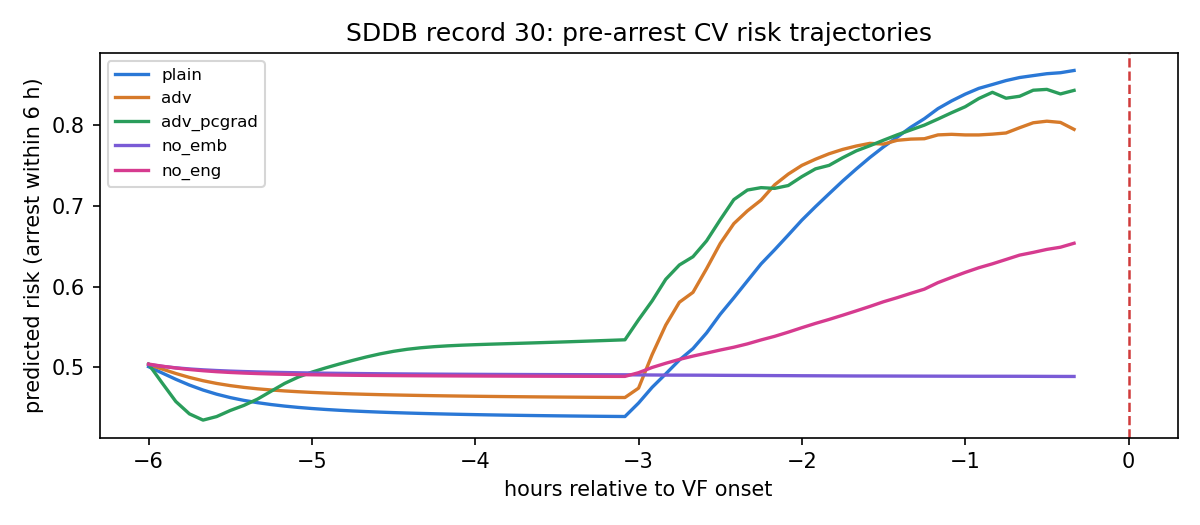
\includegraphics[width=\linewidth]{images/fig05_sddb_trajectory.png}
\caption{Cross validated risk trajectories for one real patient, hours relative
to ventricular fibrillation onset. The predicted risk does not rise before the
real event in any variant.}
\label{fig:sddb}
\end{figure}

\begin{figure}[t]
\centering
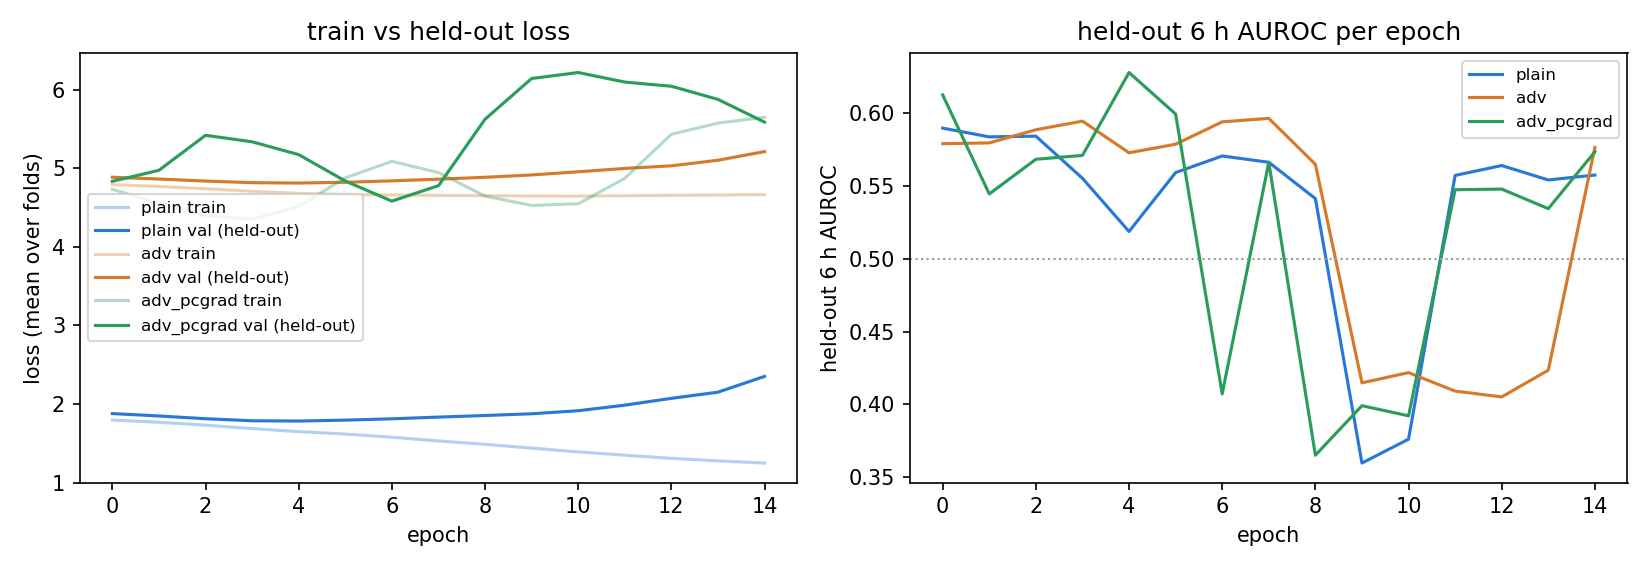
\includegraphics[width=\linewidth]{images/fig06_sddb_curves.png}
\caption{Train versus held out loss per epoch (mean over folds) for the three
identity adversarial variants, and held out 6 hour AUROC per epoch.}
\label{fig:curves}
\end{figure}

\begin{figure}[t]
\centering
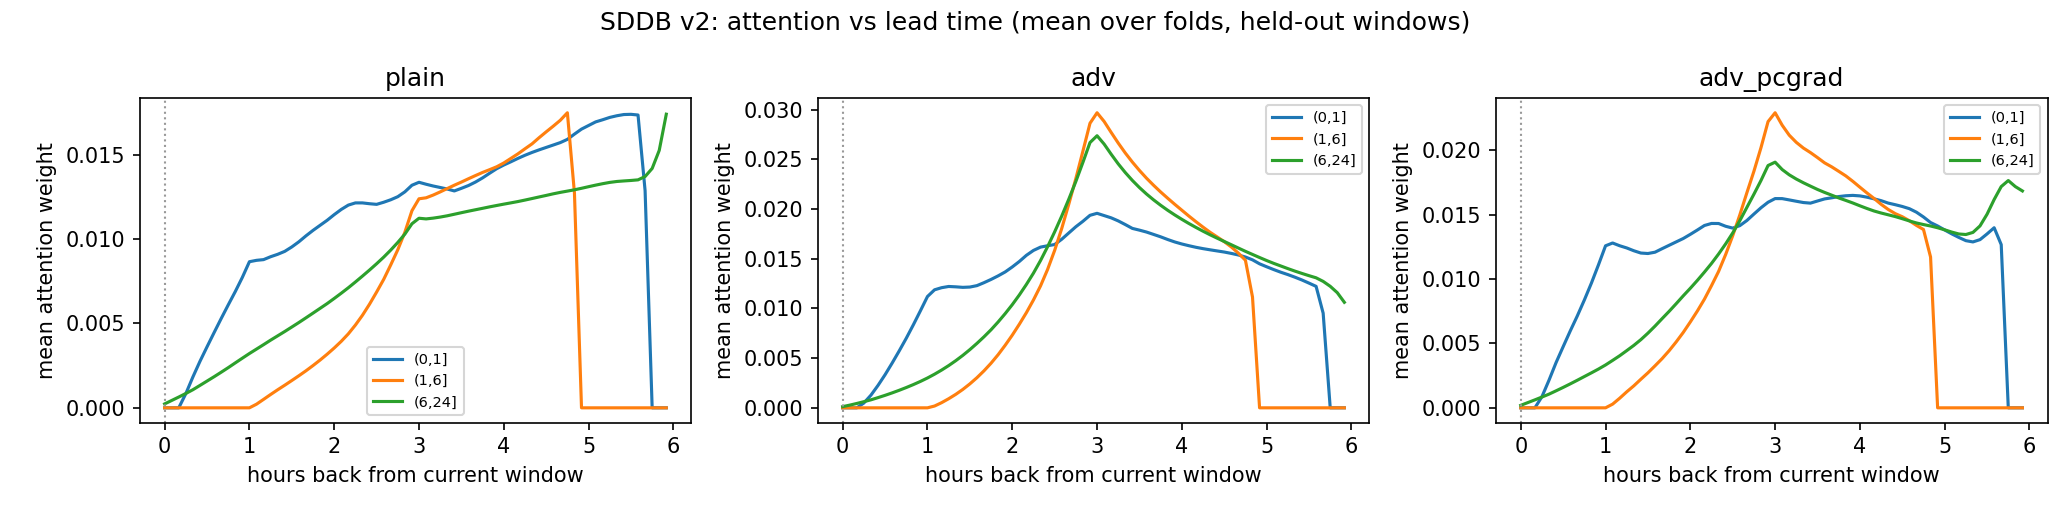
\includegraphics[width=\linewidth]{images/fig07_sddb_attention.png}
\caption{Attention salience by lead time bin (mean over folds): the model
spreads attention over history and puts near zero weight on the current
window.}
\label{fig:attention}
\end{figure}

\subsection{Robustness}
Five perturbation families were applied to the held out replay patients and
scored with the trained models (concatenation versus mask aware gated and
weighted fusion). Waveform perturbations were re embedded through the real
encoders: ECG noise at SNR 20, 10 and 5 dB, baseline wander, 50 Hz mains,
flatline halves, saturation, and PPG noise at 5 dB. Feature level stress
covered vitals noise at 0.5 to 2 times the per column standard deviation,
missing PPG, delayed measurements shifting the whole vector by 5, 10 and 15
minutes, and a sensor failure where PPG dies mid stay. Every perturbation
lands within 0.03 of the clean 6 hour AUROC (0.929 to 0.945); the only
directional effect is the delay family, which degrades monotonically but
mildly (0.929 to 0.920 at 15 minutes). Figures~\ref{fig:robnoise} and
\ref{fig:robfail} show the sweep.

Honest caveats: this measures robustness on synthetic data, where the risk
signal lives in the vitals and engineered blocks (the earlier ablation
finding), so waveform robustness partly reflects the encoders and partly that
the embeddings matter little there; the quality gates would reject flatline
and saturation windows in the real pipeline, and these tests bypassed the
gates and still held; and with 2 replay patients these are point estimates.

\begin{figure}[t]
\centering
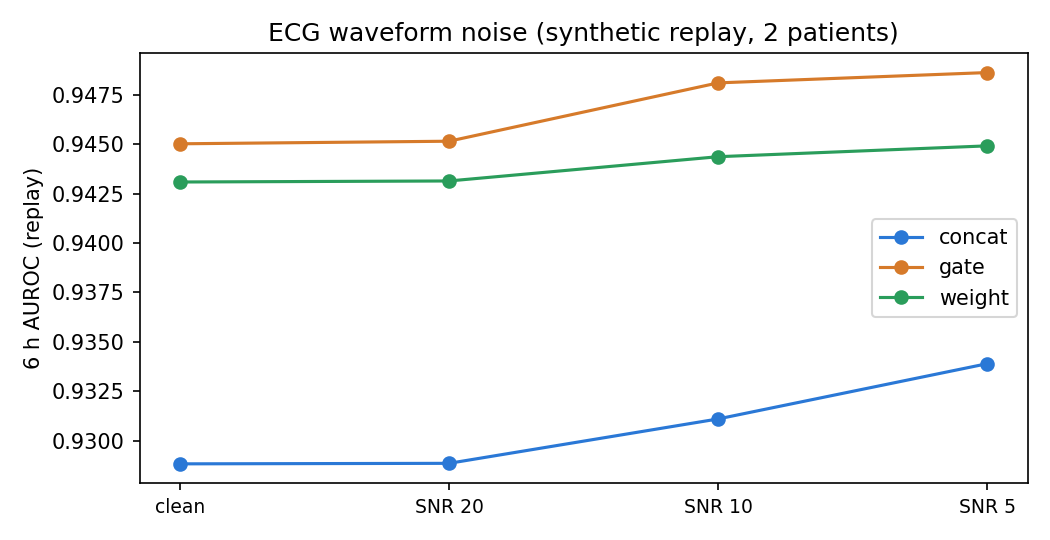
\includegraphics[width=\linewidth]{images/fig09_robustness_noise.png}
\caption{6 hour AUROC versus ECG waveform noise level (synthetic replay). No
degradation down to SNR 5 dB.}
\label{fig:robnoise}
\end{figure}

\begin{figure}[t]
\centering
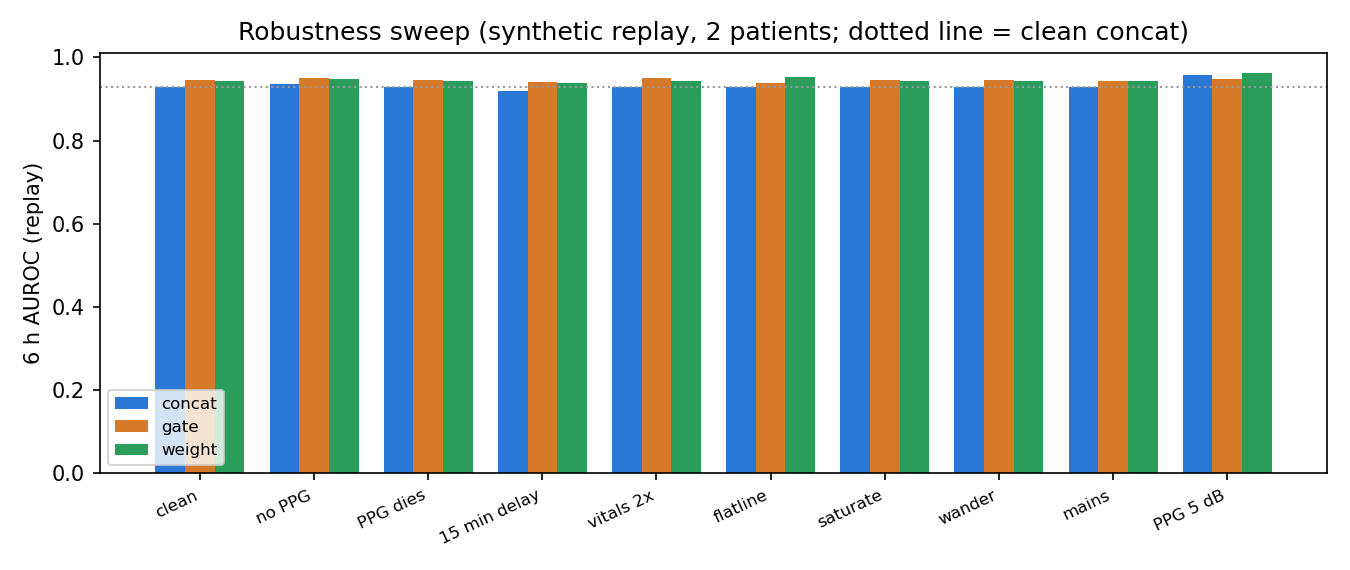
\includegraphics[width=\linewidth]{images/fig10_robustness_failure.png}
\caption{Robustness sweep across all perturbation families (synthetic replay;
the dotted line is the clean concatenation score).}
\label{fig:robfail}
\end{figure}

\section{Discussion}
Three facts explain the negative real data result. First, only 16 training
patients were available after grouping, far below what a temporal network needs to
generalize; the identity adversarial head and three alternative fusion schemes did
not change this, and a linear identity probe shows the representation still
encodes patient identity, so the overfitting mechanism is not removed by
gradient reversal. Second, the strongest modality blocks (photoplethysmogram,
arterial pressure, vitals) were absent and zero filled; missing modality masks
routed the absent photoplethysmogram to a learned embedding, which kept
predictions finite but did not recover signal. Third, Holter recordings from the
1980s differ from ICU bedside monitors, and ventricular fibrillation onset often
has no gradual electrocardiographic prodrome hours ahead, which is consistent with
the literature. The one robust hint of signal, at 1 hour, comes from engineered
rate features (heart rate variability, ectopy), not from embeddings, which
suggests that what little premonitory information exists at that horizon is
hemodynamic or rate based. This dataset therefore cannot validate a hemodynamic
early warning system; it bounds the electrocardiogram only regime, and our
results suggest that regime alone is not enough.

The decisive evaluation is the credentialed MIMIC III route: the Ext CA annotation
set (36 arrest episodes from 31 ICU patients with photoplethysmogram plus
electrocardiogram or arterial pressure) together with the waveform matched subset
provides exactly the modalities this pipeline was designed for. That evaluation is
pending access approval and will be reported separately with the same patient
level, confidence interval aware protocol.

\section{Conclusion}
We built and validated a complete multimodal early warning pipeline, and stressed
it against the only open access real pre arrest dataset. The machinery is sound
and reproducible; the synthetic benchmark is passed; the real data test fails at
6 hours for every model variant we tried, which correctly scopes the problem.
The electrocardiogram alone, in a Holter regime with 20 patients, does not carry
the 6 hour signal this model needs, and the only robust hint of signal, at 1 hour,
comes from engineered rate features. The next and decisive step is the
credentialed ICU evaluation with full modalities.

\section{Reproducibility}
Code is available as a single notebook with supporting scripts. Embedding models:
ECG FM (repository commit 9f926f19, official Hugging Face release) and PaPaGei S
(repository commit 0c537dad, Zenodo record 13983110). Real data: Sudden Cardiac
Death Holter Database version 1.0.0 on PhysioNet (open access). All metrics,
figures and configuration are exported with the run; seeds are fixed; every
expensive step is cached; no patient appears in more than one split.

\end{document}